\chapter{Теоретические основы автоматизации процесса работы наземных транспортно-технологических средств}\label{ch:ch1}

\section{Обзор текущего состояния автоматизации в сфере наземных транспортно-технологических средств}\label{sec:ch1/sec1}

\subsection{Определение автоматизации}\label{subsec:ch1/sec1/sub1}

Формирование автоматики как самостоятельной отрасли науки и техники сопровождалось установлением определенных общепринятых понятий. Определенность понятий и их точное понимание имеют важное значение, так как методы и средства автоматики нашли широкое применение в различных отраслях народного хозяйства.

Автоматика -- отрасль науки и техники об управлении и контроле протекания различных процессов, действующих без непосредственного участия человека. Более конкретное (узкое) определение автоматики -- это совокупность методов и технических средств, исключающих участие человека при выполнении операций конкретного процесса.

Автоматизация -- процесс, при котором функции управления и контроля осуществляются методами и средствами автоматики. В применении к любому производству автоматизация характеризуется освобождением человека от непосредственного выполнения функций управления производственными процессами и передачей этих функций автоматическим устройствам. Понятие автоматизации имеет широкое содержание, включающее комплекс технических, экономических и социальных вопросов. Техническая направленность автоматизации позволяет организовать технологические процессы с такой скоростью, точностью, надежностью и экономичностью, которые человек обеспечить не может. Экономическая направленность позволяет получить сравнительно быструю окупаемость первоначальных затрат за счет снижения эксплуатационных расходов и повышения объема и качества выпускаемой продукции, а социальная направленность позволяет изменить характер и улучшить условия труда человека.

По степени автоматизации производства различают частичную, комплексную и полную автоматизацию.

Частичная автоматизация -- это автоматическое выполнение отдельных производственных операций, осуществляемое в тех случаях, когда определенные технологические процессы вследствие своей сложности или быстродействия невыполнимы для человека. Функции человека при частичной автоматизации определяются технологическим процессом и сводятся к участию в производственных операциях, контроле и управлении. Частично автоматизируется, как правило, действующее производственное оборудование, причем наиболее эффективно автоматизировать технологический процесс, который сравнительно легко можно функционально выделить из общего производства.

Комплексная автоматизация -- автоматическое выполнение всех основных производственных операций участка, цеха, завода, электростанции и т. д. как единого взаимосвязанного комплекса. Функции человека при комплексной автоматизации ограничиваются контролем и общим управлением. При комплексной автоматизации отдельные автоматические регуляторы и программные устройства должны быть связаны между собой, и образовывать единую систему управления.

Полная автоматизация -- высшая ступень, при которой автоматизируются все основные и вспомогательные участки производства, включая систему управления и контроля. Управление и контроль автоматизируются с помощью вычислительных машин или специализированных автоматических устройств. Функции человека при полной автоматизации сводятся к наблюдению за работой оборудования и устранению возникающих неисправностей.

При определении степени автоматизации следует учитывать прежде всего экономическую эффективность и техническую целесообразность в условиях конкретного производства.

В зависимости от выполняемых функций автоматизация классифицируется на следующие основные виды: управление, контроль, сигнализация, блокировка, защиты и регулирование.

Управление -- это совокупность действий, направленных на поддержание функционирования объекта в соответствии с заданной программой, выполняемых на основе определенной информации о значениях параметров управляемого процесса (приведенное определение термина «управление» имеет в основном технический смысл применительно к изучаемому предмету).

Любой процесс управления в каждый момент времени характеризуется одним или несколькими показателями, которые отражают физическое состояние управляемого объекта (температура, скорость, давление, электрическое напряжение, ток, электромагнитное поле и т. д.). Эти показатели в процессе управления должны изменяться по какому-либо закону или оставаться неизменными при изменении внешних условий и режимов работы управляемого устройства. Такие показатели называются параметрами управляемого процесса.

С точки зрения автоматизации производства управление разделяется на автоматическое и полуавтоматическое.

При автоматическом управлении подача команд на управляемый объект осуществляется от специальных устройств либо по заданной программе, либо на основании информации контролируемых параметров. При полуавтоматическом управлении контроль работы управляемого объекта и подачи команд осуществляется частично оператором. Полуавтоматическое управление может быть местным или дистанционным. При местном управлении аппараты управления и контроля размещаются рядом с объектом, при дистанционном -- на любом расстоянии от объекта.

Автоматический контроль -- автоматическое получение и обработка информации о значениях контролируемых параметров объекта с целью выявления необходимости управляющего воздействия. Автоматический контроль можно рассматривать как составную часть автоматического управления, так как для протекания процесса по заданной программе необходимо иметь информацию о значениях контролируемых параметров, с тем чтобы оказывать при необходимости управляющее воздействие. Контроль может быть непрерывным и дискретным. Непрерывный контроль -- это контроль, при котором контролируемые параметры постоянно сопоставляются с заданными значениями. Дискретный контроль -- это контроль, при котором сопоставление параметров осуществляется периодически. Контроль также классифицируется на местный и дистанционный. Местный контроль -- это контроль, при котором наблюдение за состоянием параметров осуществляется непосредственно у объекта, при дистанционном контроле наблюдение за состоянием параметров осуществляется на расстоянии от объекта.

Сигнализация -- это преобразование информации о функционировании контролируемого объекта (о значении характерных параметров) в условный сигнал, понятный дежурному или обслуживающему персоналу. Сигнализация обычно разделяется на технологическую и аварийную. Технологическая сигнализация извещает персонал о ходе процесса при возможных допустимых отклонениях контролируемых параметров. Извещение может быть в виде световых сигналов (загорание или мигание ламп, табло и т. д.), а также сочетанием световых и звуковых сигналов. Аварийная сигнализация извещает об отклонениях контролируемых параметров технологического процесса за допустимые пределы и необходимость вмешательства персонала. Аварийное извещение должно отличаться от .технологического по своему логическому восприятию. Обычно оно выполняется в виде световых и звуковых сигналов.

Пример технологической и аварийной сигнализации -- это функционирование релейной защиты электрической станции. При заданных значениях напряжения и тока постоянно горящее световое табло свидетельствует о нормальном режиме работы высоковольтного оборудования. При отклонении напряжения и тока электрической сети за допустимые значения срабатывает релейная защита и световое табло начинает мигать в сопровождении звуковых прерывистых сигналов.

Блокировка -- это фиксация механизмов, устройств в определенном состоянии в процессе их работы. Блокировка позволяет сохранить механизм, устройство в фиксированном положении после получения внешнего воздействия. Блокировка повышает безопасность обслуживания и надежность работы оборудования, обеспечивает требуемую последовательность включения механизмов, устройств, а также ограничивает перемещение механизмов в пределах рабочей зоны. Примером блокировки может служить устройство высоковольтного выключателя. Механизм блокировки устроен таким образом, что включение выключателя возможно только при закрытой лицевой панели.

Автоматическая защита -- это совокупность методов и средств, прекращающих процесс при возникновении отклонений за допустимые значения контролируемых параметров. Так, например, при перегрузках или коротких замыканиях в электрических сетях происходит срабатывание определенного вида защиты (тепловой, максимального тока и т. д.) и автоматическое отключение аварийных участков. В ряде случаев устройства защиты одновременно выполняют функции управления. Например, для повышения уровня бесперебойности электроснабжения защитные устройства с одновременным отключением аварийной цепи автоматически включают резервные цепи.

Автоматическое регулирование -- это автоматическое обеспечение заданных значений параметров, определяющих требуемое протекание управляемого процесса в соответствии с установленной программой. Автоматическое регулирование можно рассматривать как составную часть автоматического управления.

Параметры управляемого процесса, подлежащие заданным изменениям или стабилизации, называют регулируемыми параметрами.

Устройство, аппарат или изделие, у которых регулируются один или несколько параметров, называют объектом автоматического регулирования.

Устройство, обеспечивающее автоматическое поддержание заданного значения регулируемого параметра в управляемом объекте или его изменения по определенному закону, называют регулятором.

Совокупность объекта регулирования и автоматического регулятора называют системой автоматического регулирования (САР).

В системе автоматического регулирования различают прямую и обратную связь.

Прямая связь -- это воздействие каждого предыдущего элемента регулятора на последующий.

Обратная связь -- воздействие одного из последующих элементов регулятора на предыдущий. Обратная связь бывает положительной, когда направление ее воздействия совпадает с направлением воздействия предыдущего элемента на последующий, и отрицательной в противоположном случае.

Автоматизация — применение технических средств, экономико-математических методов и систем управления, освобождающих человека частично или полностью от непосредственного участия в процессах получения, преобразования, передачи и использования энергии, материалов или информации.

\subsection{Роль и значение автоматизации для эффективности работы}\label{subsec:ch1/sec1/sub2}

Роль

\section{Основные принципы автоматизации процесса работы наземных транспортно-технологических средств}\label{sec:ch1/sec2}

\subsection{Системы управления и контроля}\label{subsec:ch1/sec2/sub1}

По степени автоматизации различают машины с механизированным управлением, с автоматизированным управлением и контролем на базе микропроцессорной техники, с автоматизированным управлением на расстоянии, с автоматическим управлением на базе микропроцессоров и мини-ЭВМ, строительные манипуляторы и роботы, а также роботизированные машины и комплексы \cite[с.~39]{Evtukov}.

Системы управления предназначены для включения и выключения различных механизмов машин \cite[с.~109]{Evtukov}.
По назначению системы управления можно разделить на следующие: управлением двигателем; управление муфтами и тормозами; рулевое управление; управление рабочим органом (например, опускание и подъем отвала бульдозера или ковша скрепера, поворот отвала автогрейдера).

По конструкции системы управления строительных машин разделяют на механические, гидравлические, пневматические, электрические и смешанные (комбинированные), аналогично силовым приводам, но в отличие от которых в большинстве случаев в системах управления передаются значительно меньше силы.

Различают машины с механизированным и автоматизированным управлением. Автоматизированное управление и контроль рабочего процесса могут осуществляться на базе микропроцессоров и мини-ЭВМ, а также строительные манипуляторы и роботы, роботизированные машины и комплексы.

\subsection{Использование датчиков и сенсоров}\label{subsec:ch1/sec2/sub2}

С помощью различных датчиков обеспечивается сбор данных о состоянии окружающей среды. Датчики можно классифицировать на датчики внешней информации и внутренней \cite[с.~131]{Vlasov}. 

Датчики внутренней информации представляют собой в основном преобразователи механических параметров в электрические сигналы. Например датчики обратной связи по положению, скорости и ускорения.

\begin{figure}[ht]
    \centerfloat{
        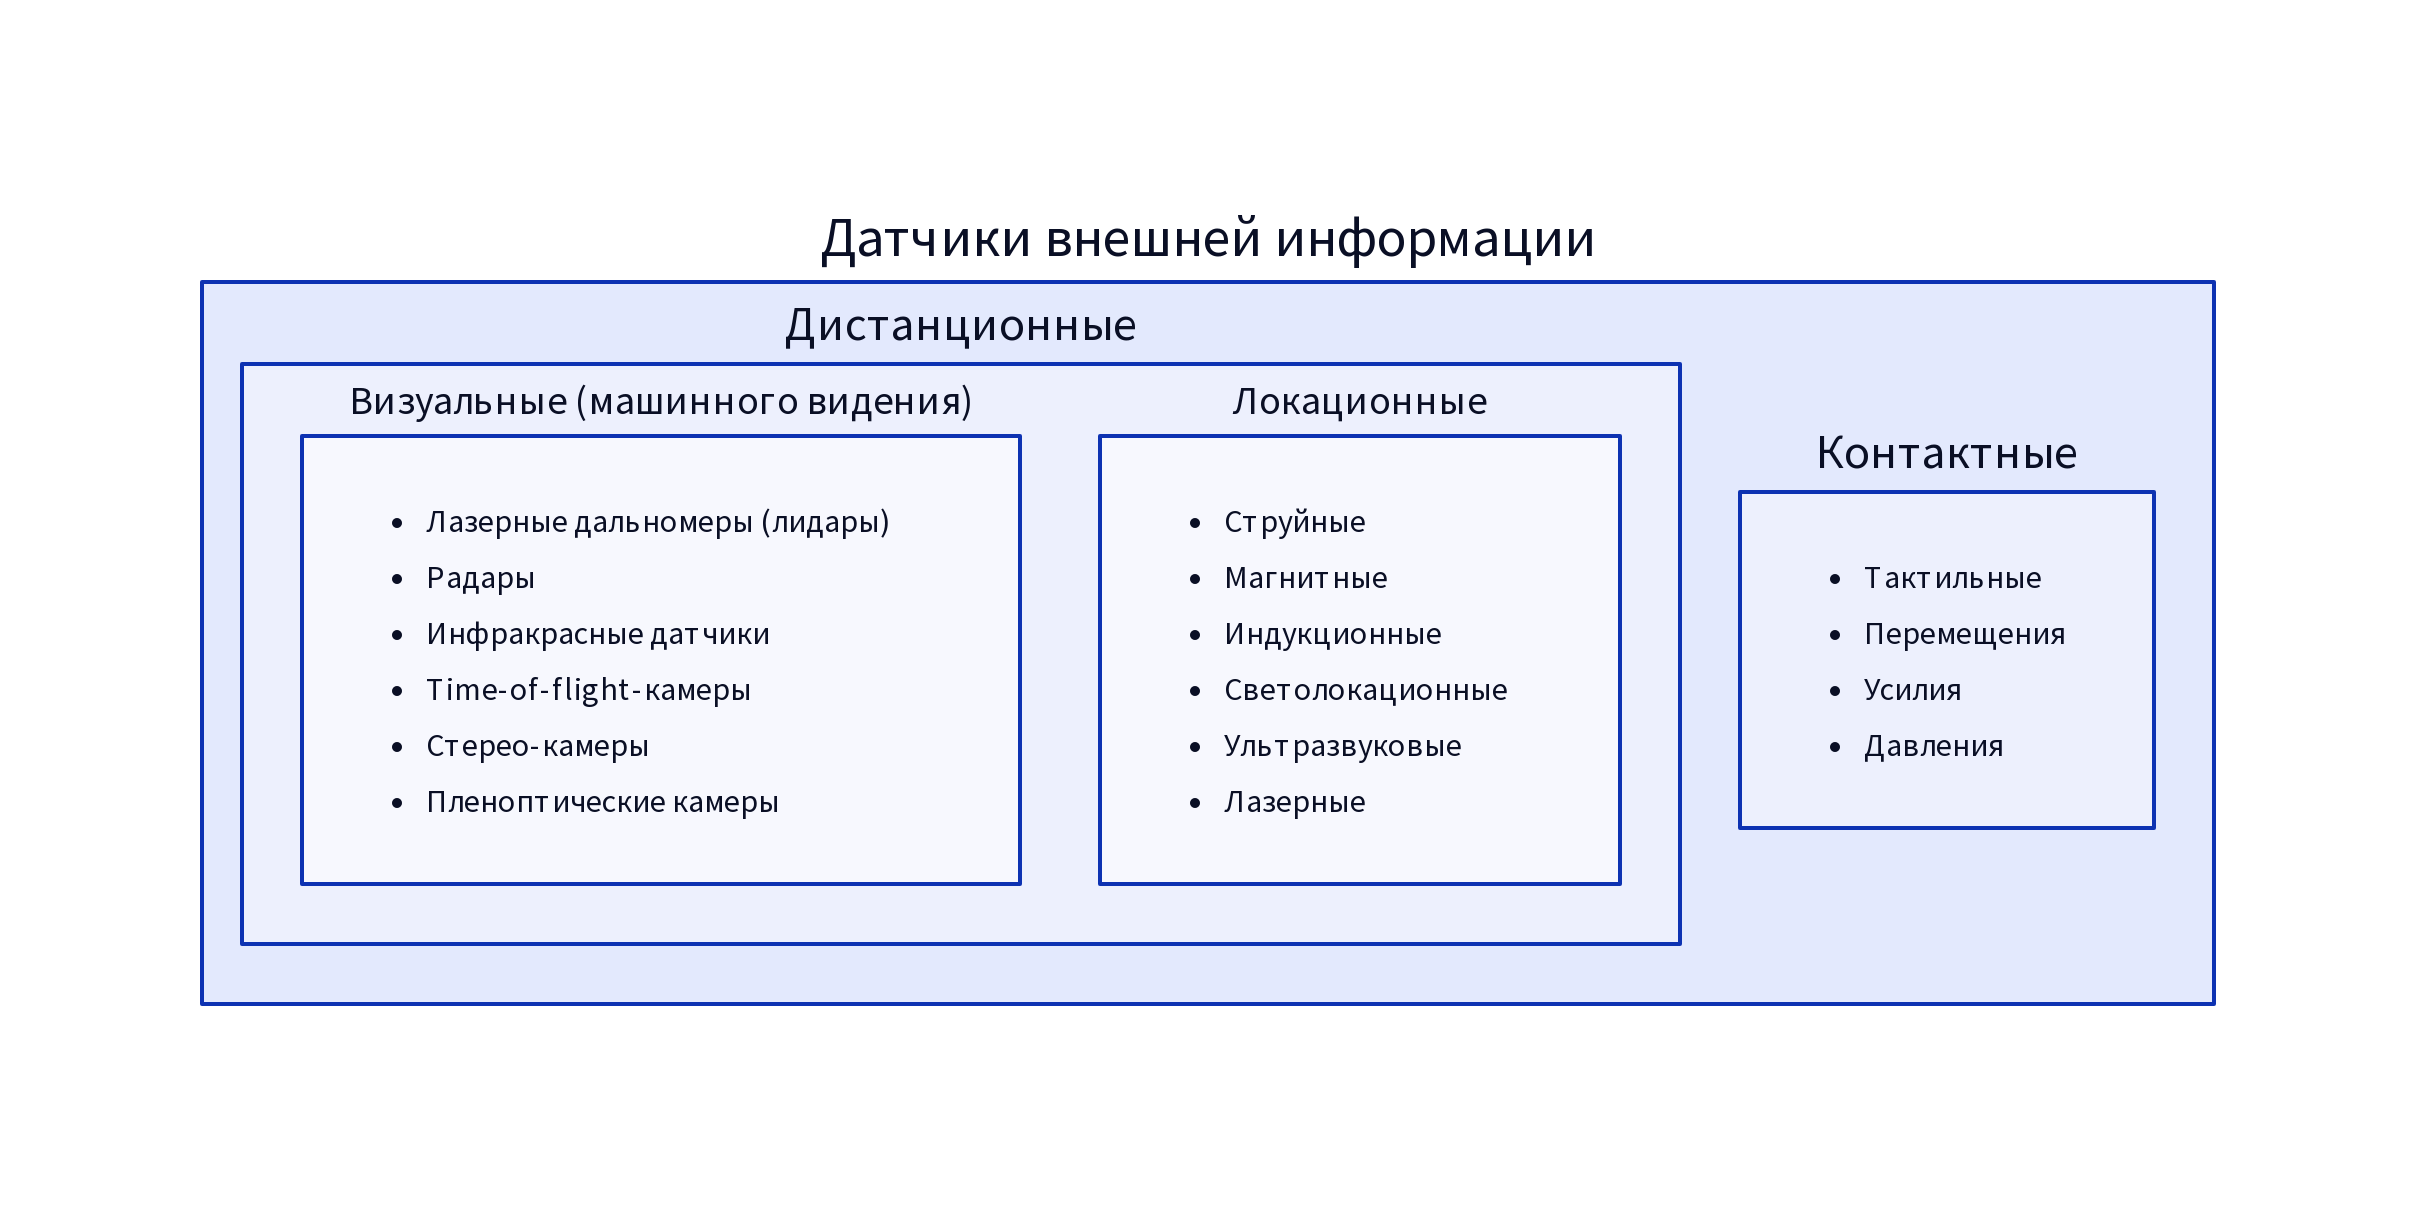
\includegraphics[scale=0.2]{d2/datchiki}
    }
    \caption{Классификация датчиков внешней информации}\label{fig:datchiki}
\end{figure}

Датчики внешней информации обеспечивают сбор информации об окружающем мире. Их можно разделить на две большие группы (рис.~\cref{fig:datchiki}): дистанционные и контактные. В свою очередь дистанционные датчики можно разделить на локационные и визуальные.

Локационные системы можно условно разделить на два класса: дальней и ближней локации. Первые могут быть построены с использованием ультразвуковых, лазерных и светолокационных датчиков.

Визуальные системы (технического, машинного зрения) относятся к числу наиболее сложных, но и наиболее универсальных средств очувствления НТТС \nomenclature{НТТС}{наземные транспортно-технологические средства\nomrefpage}
(рис.~\cref{fig:kamaz},~\cref{fig:robot1},~\cref{fig:robot2},~\cref{fig:sensors}).

\begin{figure}[ht]
    \centerfloat{
        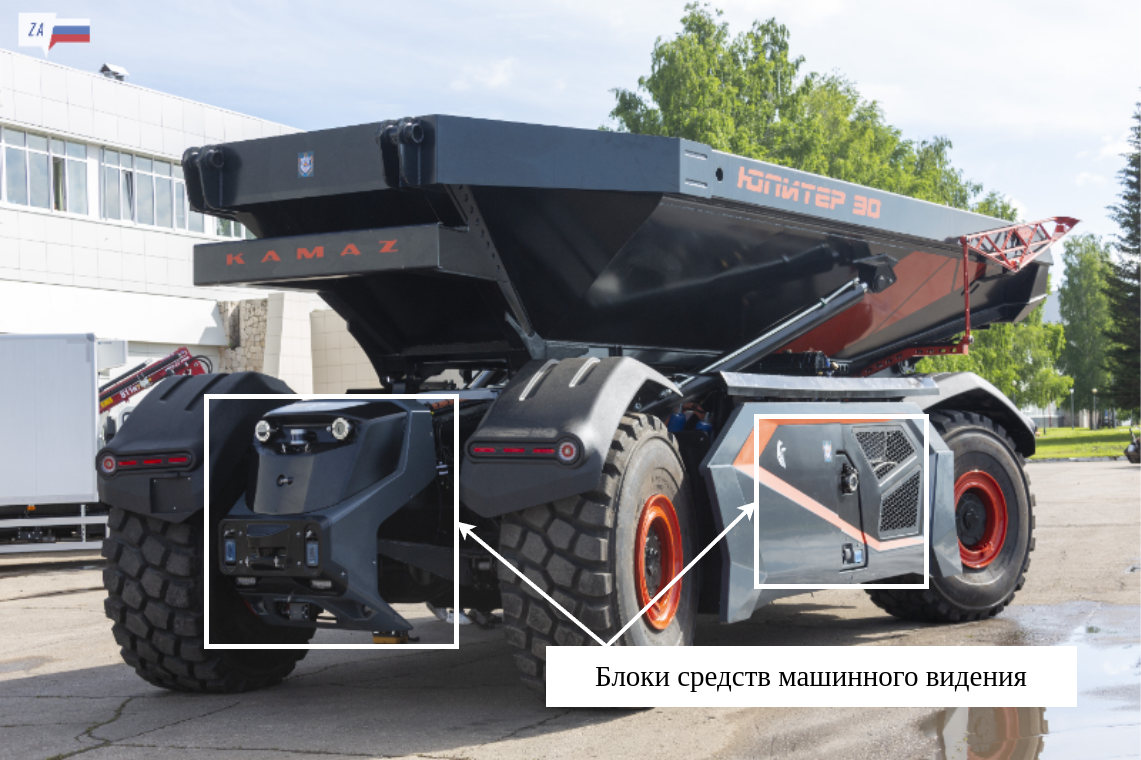
\includegraphics[scale=0.2]{views/kamaz.png}
    }
    \caption{Набор датчиков «Юпитер-30» ПАО «КАМАЗ»}\label{fig:kamaz}
\end{figure}

\begin{figure}[ht]
    \centerfloat{
        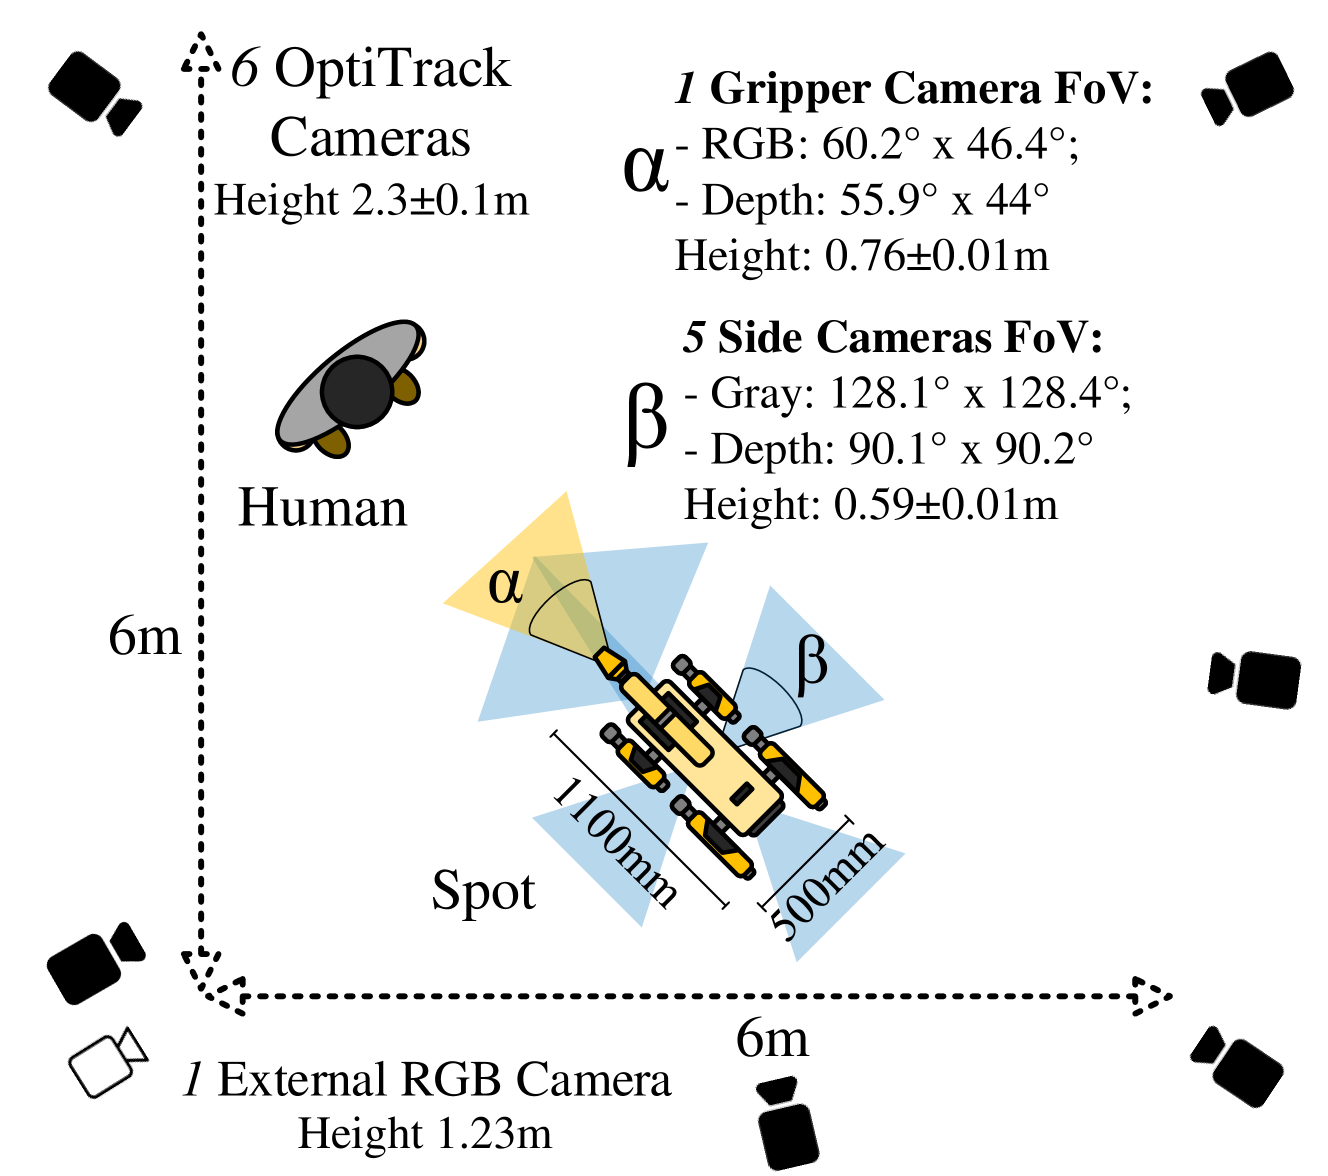
\includegraphics[scale=0.2]{views/robot1.png}
    }
    \caption{Набор датчиков автономного робота}\label{fig:robot1}
\end{figure}

\begin{figure}[ht]
    \centerfloat{
        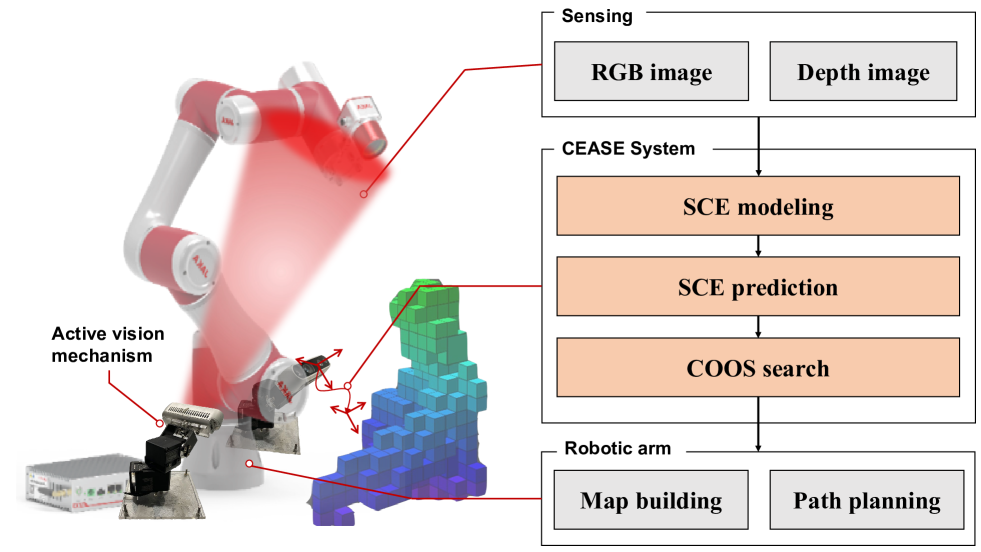
\includegraphics[scale=0.2]{views/robot2.png}
    }
    \caption{Набор датчиков робота}\label{fig:robot2}
\end{figure}

\begin{figure}[ht]
    \centerfloat{
        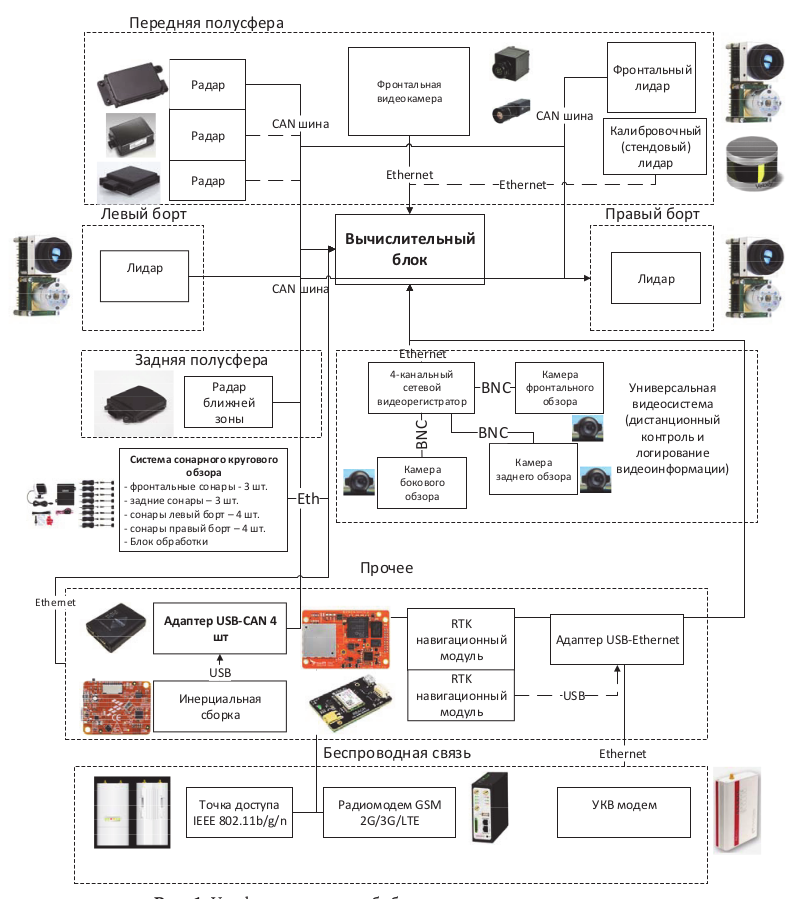
\includegraphics[scale=0.6]{views/sensors.png}
    }
    \caption{Унифицированная схема взаимосвязи датчиков}\label{fig:sensors}
\end{figure}


Основными используемыми средствами машинного видения являются~\cite{confbib1}:

Лазерные дальномеры (лидары), которые измеряют расстояние до объектов. Результат работы лидара – объемная сцена из облака точек с геометрией объектов. Это средство выдает наибольшую точность, лучше всех работают на ровных поверхностях и почти не засвечиваются солнцем. При этом имеют высокое энергопотребление, относительно низкую частоту кадров, бегущий затвор и необходимость компенсировать его при обработке, а также работающие рядом лидары создают друг-другу помехи, которые не так просто компенсировать.

Радары для определения расстояния до объекта, его скорости и месторасположения. Радары меньше зависят от погоды и стоят намного дешевле лидаров. Главным отрицательным качеством является то, что плохо обнаруживаются неметаллические объекты, в том числе пешеходы.

Инфракрасные датчики для реагирования на фоновое инфракрасное излучение. Прибор регистрирует любое тепловое излучение.

Time-of-flight-камеры (ToF\nomenclature{ToF}{Time-of-flight-камеры\nomrefpage}) - видеокамеры, формирующие дальностное изображение. Используются для создания изображений, которые в качестве пикселей содержат оценки расстояний от экрана до конкретных точек наблюдения.

Стерео-камеры, построенные на имитации бинокулярного зрения человека с возможностью захватывать трехмерные изображения.

Пленоптические камеры, фиксирующие векторное поле световых лучей (световое поле). На основе картины светового поля может быть воссоздана наиболее полная информация об изображении, пригодная для решения различных задач компьютерной графики.

Обычные камеры с последующим анализом видео-потока с применением алгоритмов машинного обучения.

Так же можно приобщить разрабатываемый метод обмена данными о местоположении, скорости, направлении движения и другими данными между объектами.

Одновременно с этим, применение какого-либо одного средства недостаточно, так как получение комплексного видения окружающего мира роботами имеет сложности в виде:

\begin{itemize}
    \item темного времени суток;
    \item засветов от солнца и источников освещения;
    \item инфракрасного излучение солнечного света;
    \item осадков и грязи;
    \item множественности и вариативности подвижных окружающих объектов.
\end{itemize}

В связи с этим, средства машинного видения применяются комплексно, для компенсации недостатков друг-друга. Сравнительный анализ приведен в~таблице~\ref{tab:TableViews}.

\begin{table}[htbp]
    \centering
    \begin{threeparttable}
        \caption{Сравнительный анализ средств машинного видения}\label{tab:TableViews}%
            \begin{tabular}{{| p{3cm} || p{2cm} | p{2cm} | p{2cm} | p{2cm} | p{2cm} |}}
            \hline
            & ToF & Стерео & Пленопт. & Лидары & Радары \\ \hline
            Разрешение                 & \textit{Слабо}  & Средне & \textbf{\begin{tabular}[c]{@{}l@{}}Отлично\\ (сцена)\end{tabular}} & \begin{tabular}[c]{@{}l@{}}Средне\\ (сцена)\end{tabular} & \textit{Слабо}  \\ \hline
            Точность                    & Средне          & Средне          & \textit{Слабо}            & \textit{Слабо}  & \textbf{Высоко} \\ \hline
            Сложность ПО \nomenclature{ПО}{программное обеспечение\nomrefpage}                & \textbf{Слабо}  & Средне          & \textit{Высоко}           & \textit{Высоко} & \textbf{Слабо}  \\ \hline
            Работа в реальном времени   & \textbf{Высоко} & Средне          & Средне                    & Средне          & \textit{Слабо}  \\ \hline
            Стоимость                   & Средне          & Средне          & \textbf{Слабо}            & \textit{Высоко} & Средне          \\ \hline
            Производ-сть при слабом освещении & \textbf{Хорошо} & \textbf{Хорошо} & \textit{Плохо}            & \textit{Плохо}  & \textbf{Хорошо} \\ \hline
            Работа на открытом воздухе  & \textit{Плохо}  & \textit{Плохо}  & \textbf{Хорошо}           & \textbf{Хорошо} & \textbf{Хорошо} \\ \hline
            \end{tabular}
    \end{threeparttable}
\end{table}

Можно сделать вывод, что по разрешению лидируют пленоптические камеры, но все очень сильно зависит от сцены. По точности - лидары. По сложности обработки - «непосредственно» получают глубину только ToF и лидары. По частоте кадров конструктивно хороши ToF-камеры. При работе на открытом пространстве плохо работают ToF и камеры структурированного света.

Однозначно стоит в дальнейшем изучить и проанализировать использование совместно со средствами машинного видения такие методы, как:

\begin{itemize}
    \item определение местоположения в пространстве на основе глобальных систем позиционирования (GPS, ГЛОНАСС);
    \item получение данных от коллекторов навигационных данных (системы типа Яндекс-навигатор);
    \item заранее заложенные геопространственные данные;
    \item передачу управляющих сигналов внешними специализированными автоматизированными системами управления (по анализу данных с наружных камер наблюдения, управляющее воздействие регулятора и т.д.).
\end{itemize}


\subsection{Программное обеспечение для автоматизации}\label{subsec:ch1/sec2/sub3}

ПО

\section{Технологии автоматизации в наземном транспорте}\label{sec:ch1/sec3}

\subsection{Преимущества автоматизации для безопасности и эффективности работы}\label{subsec:ch1/sec3/sub1}

Преимущества

\subsection{Вызовы и проблемы, связанные с внедрением автоматизации}\label{subsec:ch1/sec3/sub2}

Вызовы

\subsection{Перспективы развития автоматизации в наземном транспорте}\label{subsec:ch1/sec3/sub3}

Перспективы

\section{Выводы по главе}\label{sec:ch1/sec4}

Выводы

\FloatBarrier
